\section{theorem15(the real main theorem)}
\begin{theorem}
\end{theorem}

Suppose we have a braid represented by a braid word $\omega = s_{i_1}\cdots s_{i_k}$, then on a two punctured Riemann sphere we have the natural alternating strand diagram associated to the braid word $\omega$. We can cover the diagram with $k$ generator regions and $k$ intergenerator regions.

Suppose we have a sheaf given as follows:
on the $k^{th}$ generator region the sheaf looks as follows. Let $i := i_k$

\begin{figure}[H] % Optional: [h] means here, [t] for top, [b] for bottom, [p] for page of floats
    \centering
    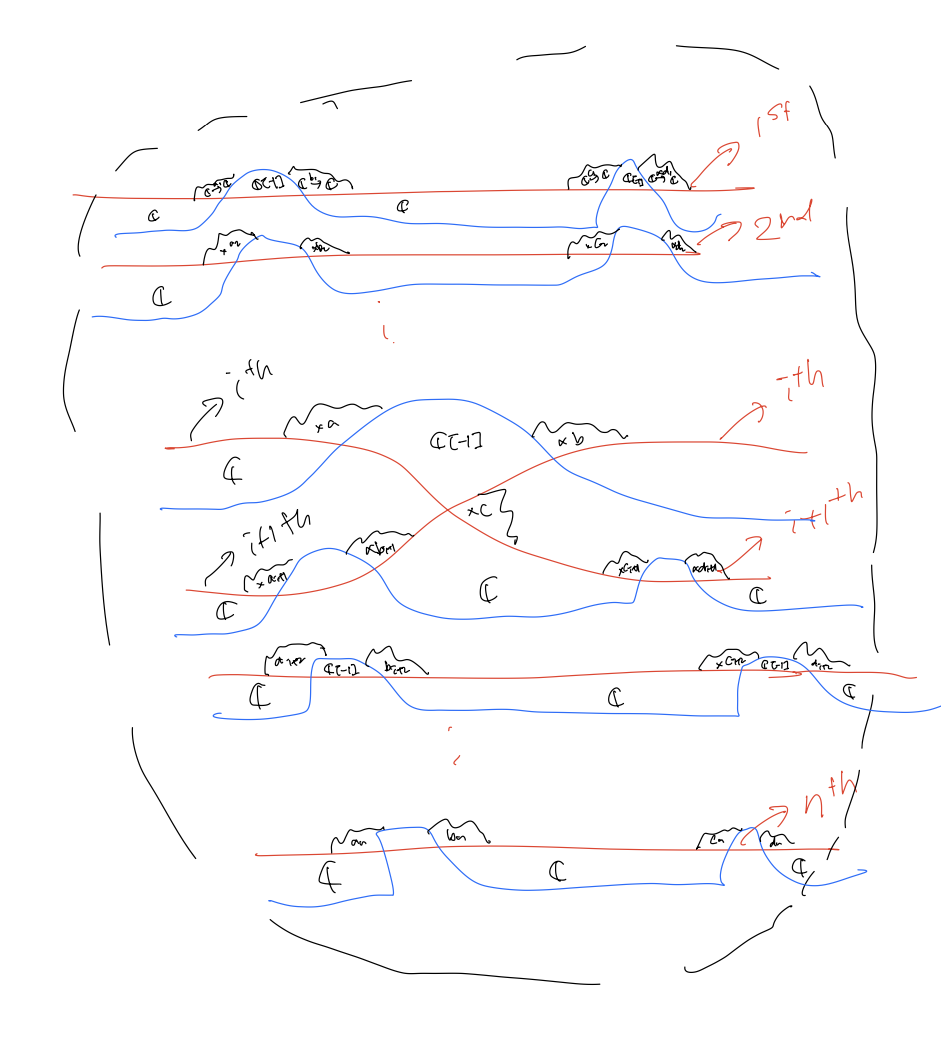
\includegraphics[width=\linewidth]{diagrams/theorem15/1.png} % Adjust the width as needed
    \caption{Your caption here}
    \label{fig:your-label}
\end{figure}

On the $k^{th}$ intergenerator region looks as follows

\begin{figure}[H] % Optional: [h] means here, [t] for top, [b] for bottom, [p] for page of floats
    \centering
    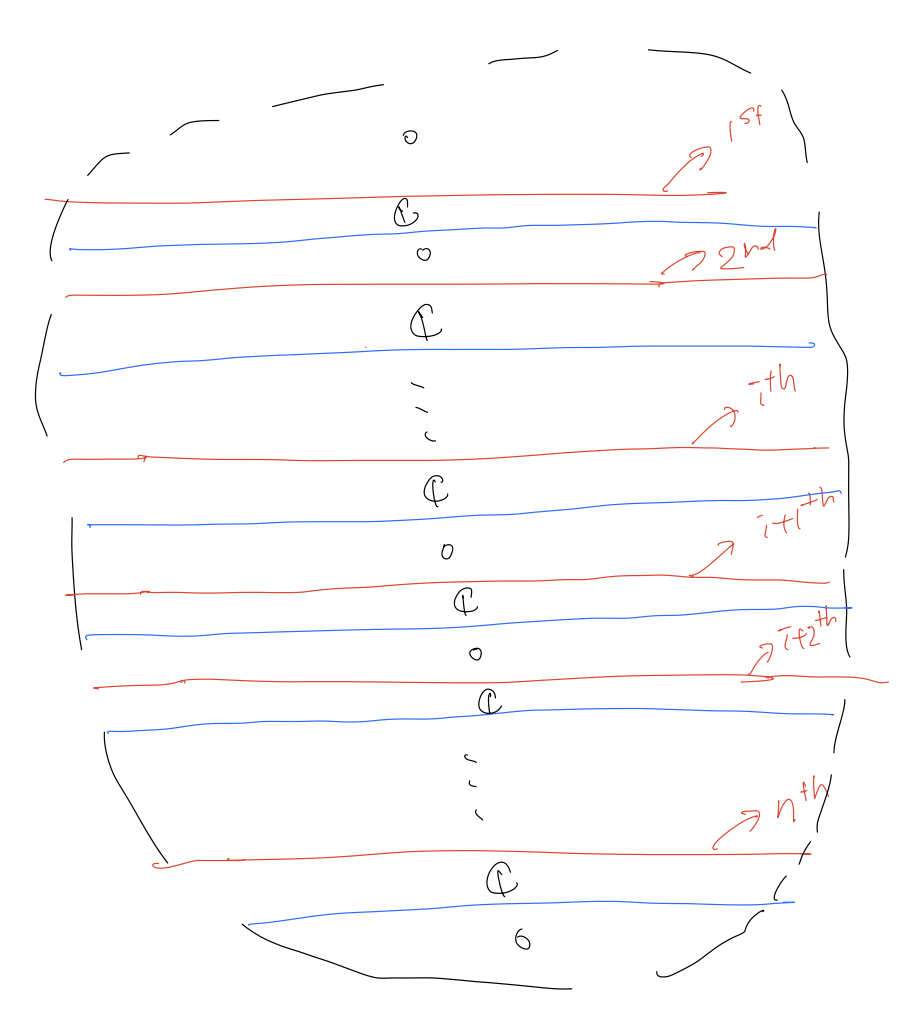
\includegraphics[width=\linewidth]{diagrams/theorem15/2.png} % Adjust the width as needed
    \caption{Your caption here}
    \label{fig:your-label}
\end{figure}

Suppose we apply MOVE \RN{12} to generator regions and then apply intergenerator moves to intergenerator regions, then we get the following sheaf :

On the $k^{th}$ generator region the sheaf looks as follows:
Let $i := i_k$
\begin{figure}[H] % Optional: [h] means here, [t] for top, [b] for bottom, [p] for page of floats
    \centering
    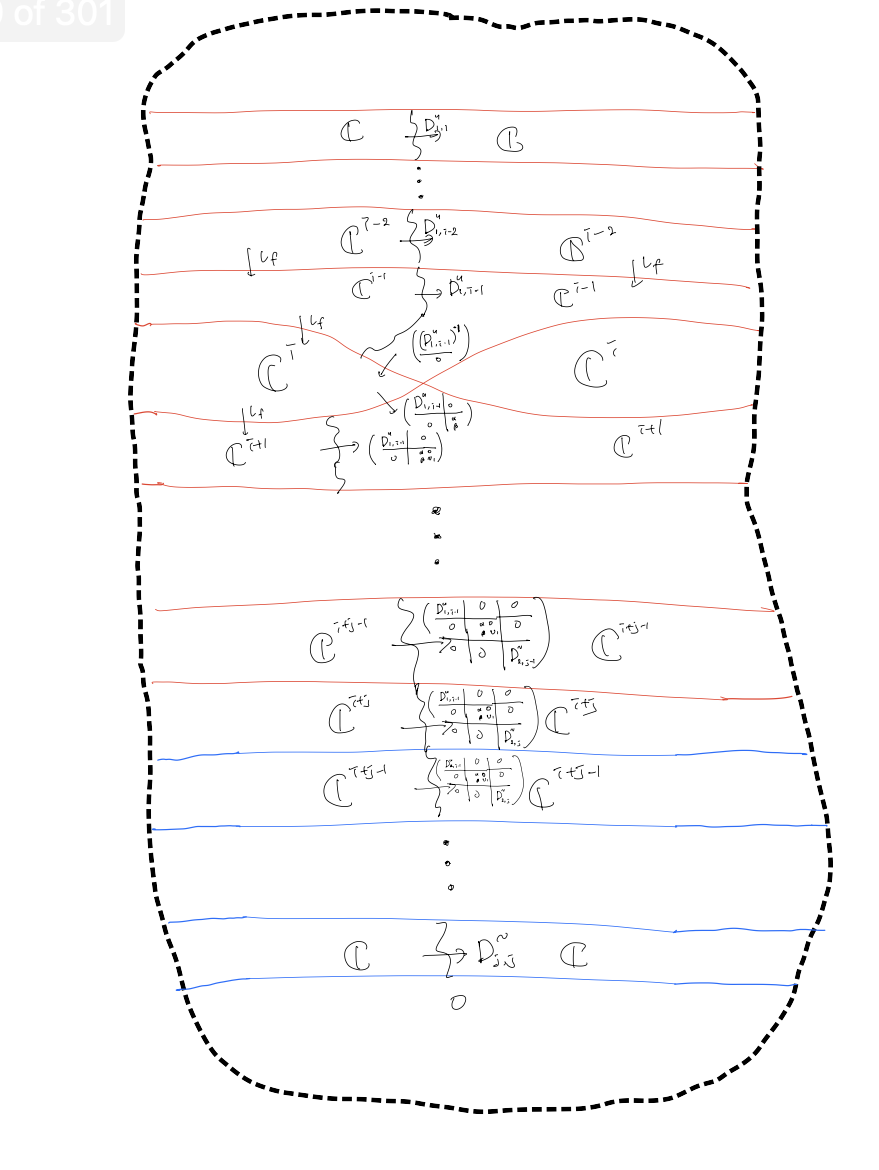
\includegraphics[width=\linewidth]{diagrams/theorem15/3.png} % Adjust the width as needed
    \caption{Your caption here}
    \label{fig:your-label}
\end{figure}

where
\begin{align*}
	& u_k := \frac{a_k\cdot c_k}{b_k\cdot d_k} (1\leq k <i)\\
	& v_k := \frac{a_k\cdot c_k}{b_k\cdot d_k} (1< k \leq n)\\
	& j := n-i
\end{align*}
and $D_{l,m}^u := diag(u_l,\cdots,u_m)$, $D_{l,m}^v := diag(v_l,\cdots,v_m)$

On the $k^{th}$ intergenerator region looks as follows :

\begin{figure}[H] % Optional: [h] means here, [t] for top, [b] for bottom, [p] for page of floats
    \centering
    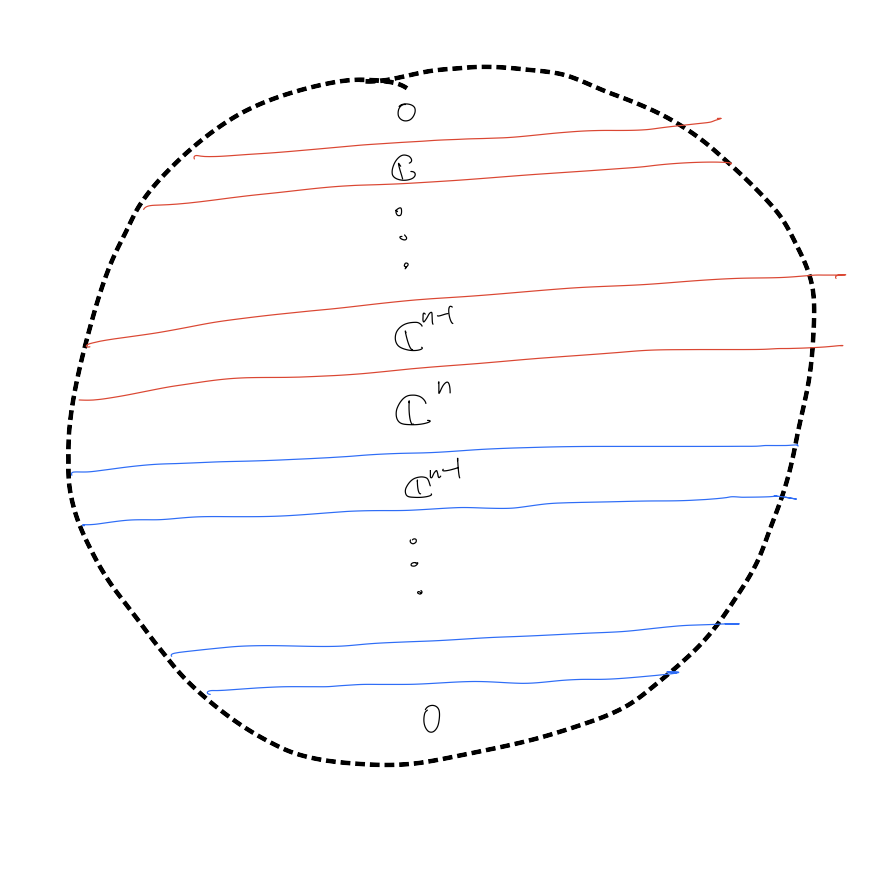
\includegraphics[width=\linewidth]{diagrams/theorem15/4.png} % Adjust the width as needed
    \caption{Your caption here}
    \label{fig:your-label}
\end{figure}
(proof) First we apply MOVE \RN{12}(generator moves) to the sheaf described above. By Lemma12, we get :
On the $k^{th}$ generator region the sheaf looks as follows :

Let $i := i_k$

\begin{figure}[H] % Optional: [h] means here, [t] for top, [b] for bottom, [p] for page of floats
    \centering
    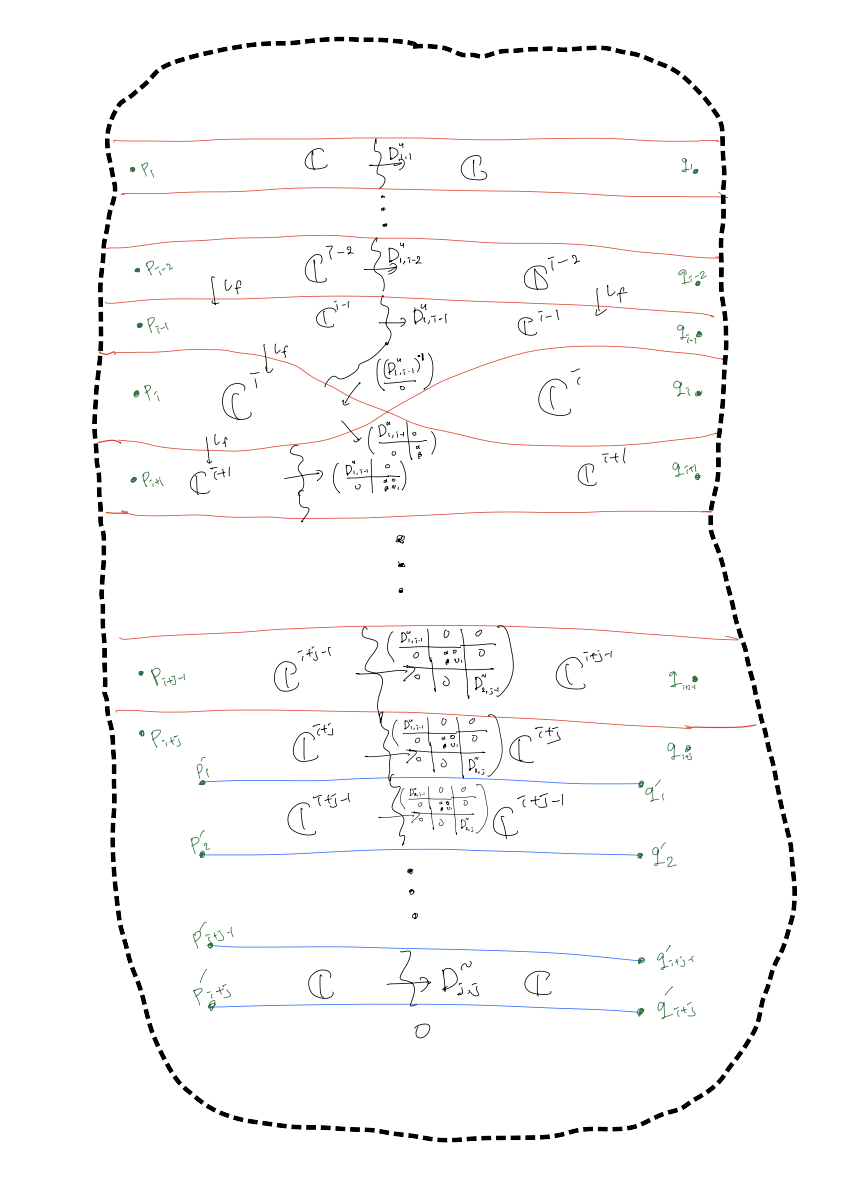
\includegraphics[width=\linewidth]{diagrams/theorem15/5.png} % Adjust the width as needed
    \caption{Your caption here}
    \label{fig:your-label}
\end{figure}

where
\begin{align*}
	& u_k := \frac{a_k\cdot c_k}{b_k\cdot d_k} (1\leq k <i)\\
	& v_k := \frac{a_k\cdot c_k}{b_k\cdot d_k} (1< k \leq n)\\
	& j := n-i
\end{align*}
and $D_{l,m}^u := diag(u_l,\cdots,u_m)$, $D_{l,m}^v := diag(v_l,\cdots,v_m)$

and the description of the intergenerator region automatically follows.

On the $k^{th}$ intergenerator region, with intergenerator sheaf on a intergenerator diagram on $n$ strands. Then we apply intergenerator move to the intergenerator regions. By the intergenerator theorem, we get :

On the $k^{th}$ generator region, the sheaf looks as follows :

Let $i:=i_k$
\begin{figure}[H] % Optional: [h] means here, [t] for top, [b] for bottom, [p] for page of floats
    \centering
    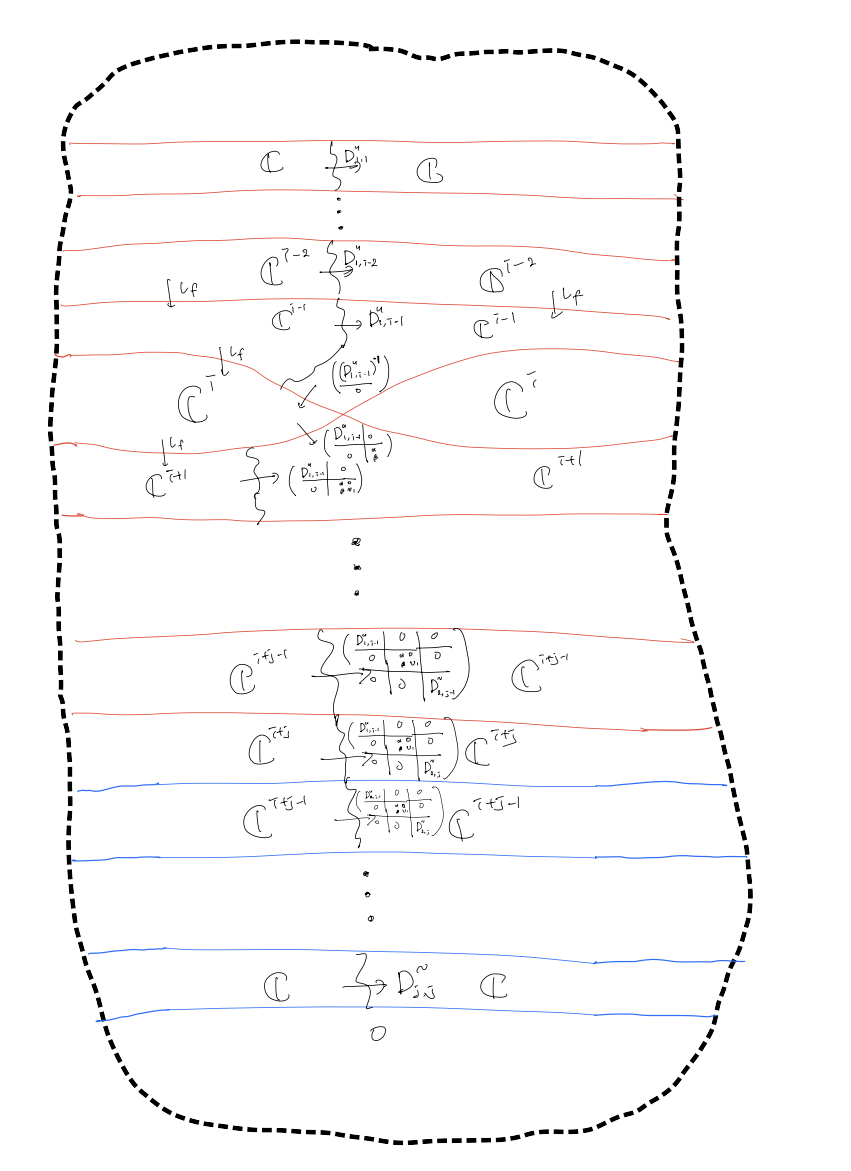
\includegraphics[width=\linewidth]{diagrams/theorem15/6.png} % Adjust the width as needed
    \caption{Your caption here}
    \label{fig:your-label}
\end{figure}

On the $k^{th}$ intergenerator region looks as follows :

\begin{figure}[H] % Optional: [h] means here, [t] for top, [b] for bottom, [p] for page of floats
    \centering
    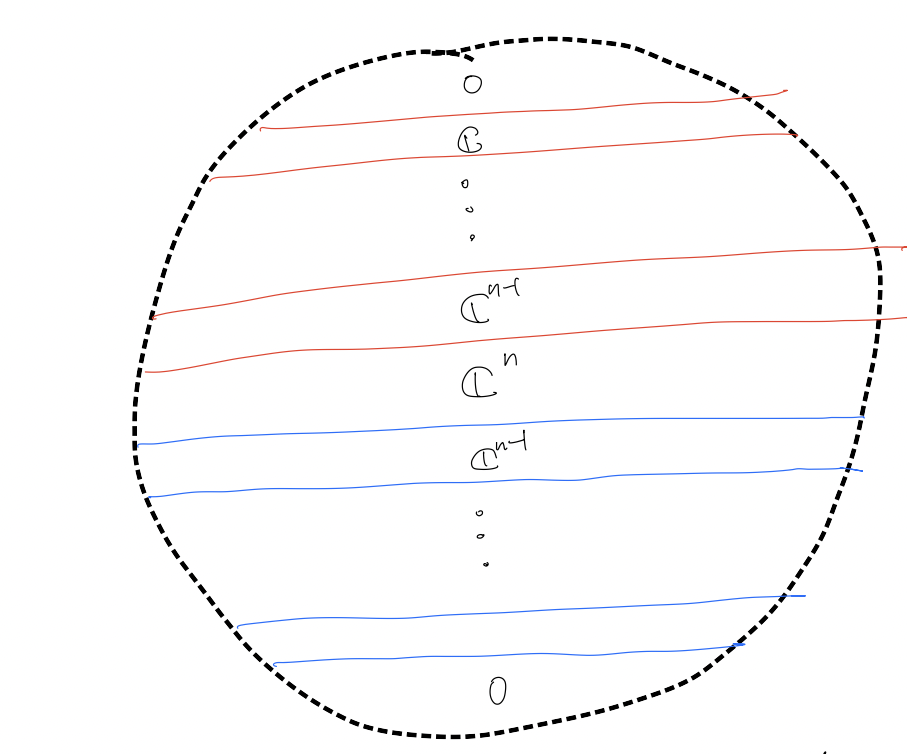
\includegraphics[width=\linewidth]{diagrams/theorem15/7.png} % Adjust the width as needed
    \caption{Your caption here}
    \label{fig:your-label}
\end{figure}